\documentclass{article}
\usepackage{epsfig}
\usepackage{hyperref}
\renewcommand{\baselinestretch}{1}
\setlength{\textheight}{9in}
\setlength{\textwidth}{6.5in}
\setlength{\headheight}{0in}
\setlength{\headsep}{0in}
\setlength{\topmargin}{0in}
\setlength{\oddsidemargin}{0in}
\setlength{\evensidemargin}{0in}
\setlength{\parindent}{.3in}
\begin{document}

\leftline{Alexander Toth}
\leftline{AME 20214}
\leftline{15 September 2016}

\medskip
This is a sample file in the text formatter \LaTeX.
I require you to use it for the following reasons:

\begin{itemize}

\item{It produces the best output of text, figures,
      and equations of any
      program I've seen.}

\item{It is machine-independent. It runs on Linux, Macintosh (see {\tt TeXShop}), and Windows (see {\tt MiKTeX} and {\tt TeXnicCenter}) machines.
     You can e-mail {\tt ASCII} versions of most relevant files.}

\item{It is the tool of choice for many research
     scientists and engineers.
     Many journals accept 
     \LaTeX~ submissions, and many books
     are written in \LaTeX.}

\end{itemize}
\medskip
Some basic instructions are given below.
Put your text in here.  You can be a little sloppy    about
spacing.  It adjusts the text to look good.
{\small You can make the text smaller.}
{\tiny You can make the text tiny.}
You can \href{http://www.nd.edu/~powers/ame.20214}{link to web sites}

Skip a line for a new paragraph.   
You can use italics ({\em e.g.} {\em  Computers are everywhere}) or {\bf bold}.
Greek letters are a snap: $\Psi$, $\psi$,
$\Phi$, $\phi$.  Equations within text are easy---
A well known equation for a line is $y=mx+b$. Here $y$ is the dependent variable, $x$ is the independent variable, $m$ is the slope, and $b$ is the intercept.
You can also set aside equations like so:
\begin{eqnarray}
{d^2 \theta \over dt^2} &=& -{g \over \ell} \sin \theta, \qquad \mbox{Newton's second law for pendulum motion}, \label{ee} \\
{g \over \ell} \sin \theta &=& {g \over \ell} \sum_{n=0}^\infty (-1)^{n} {\theta^{2n+1} \over (2n+1)!} =
{g \over \ell} \left( \theta - {\theta^3 \over 6} + {\theta^5 \over 120} - {\theta^7 \over 5040} + \dots \right). \label{e1}
\end{eqnarray}
Equation~(\ref{ee}) is Newton's second law for pendulum motion.  Here $\theta$ is the angular position, $t$ is time, $g$ is gravitational acceleration, and $\ell$ is length.   Equation~({\ref{e1}) gives a series expansion relevant to Eq.~(\ref{ee}).
References\footnote{Lamport, L., 1986, {\em \LaTeX: User's Guide \& Reference Manual},
    Addison-Wesley: Reading, Massachusetts.}
are available. 
If you have a postscript file, say {\tt sample.figure.eps}, in the same local directory,
you can insert the file as a figure.  Figure \ref{sample}, below, plots Bessel functions, three times repeated, so as to demonstrate how to insert multiple plots. 
\begin{figure}[ht]
\begin{center}
$\begin{array}{ccc}
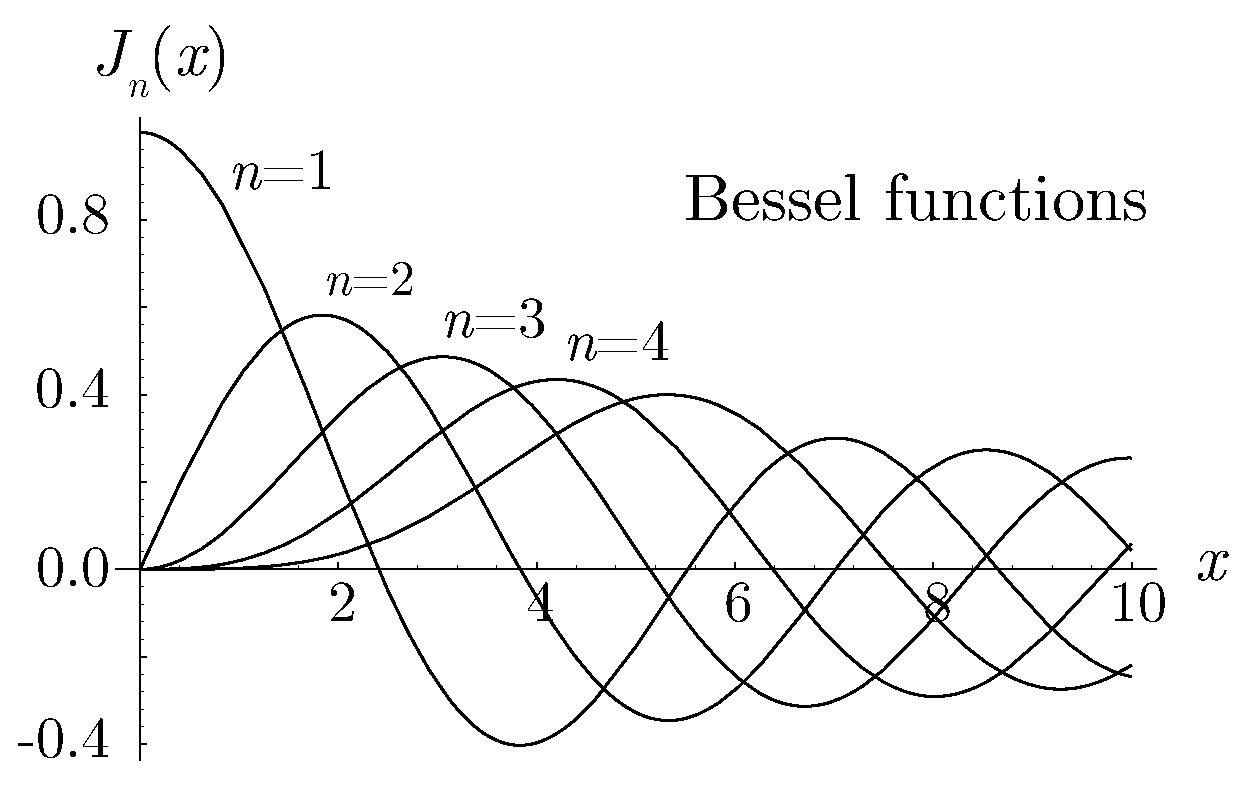
\includegraphics[width=2.0in]{sample.figure.eps} &
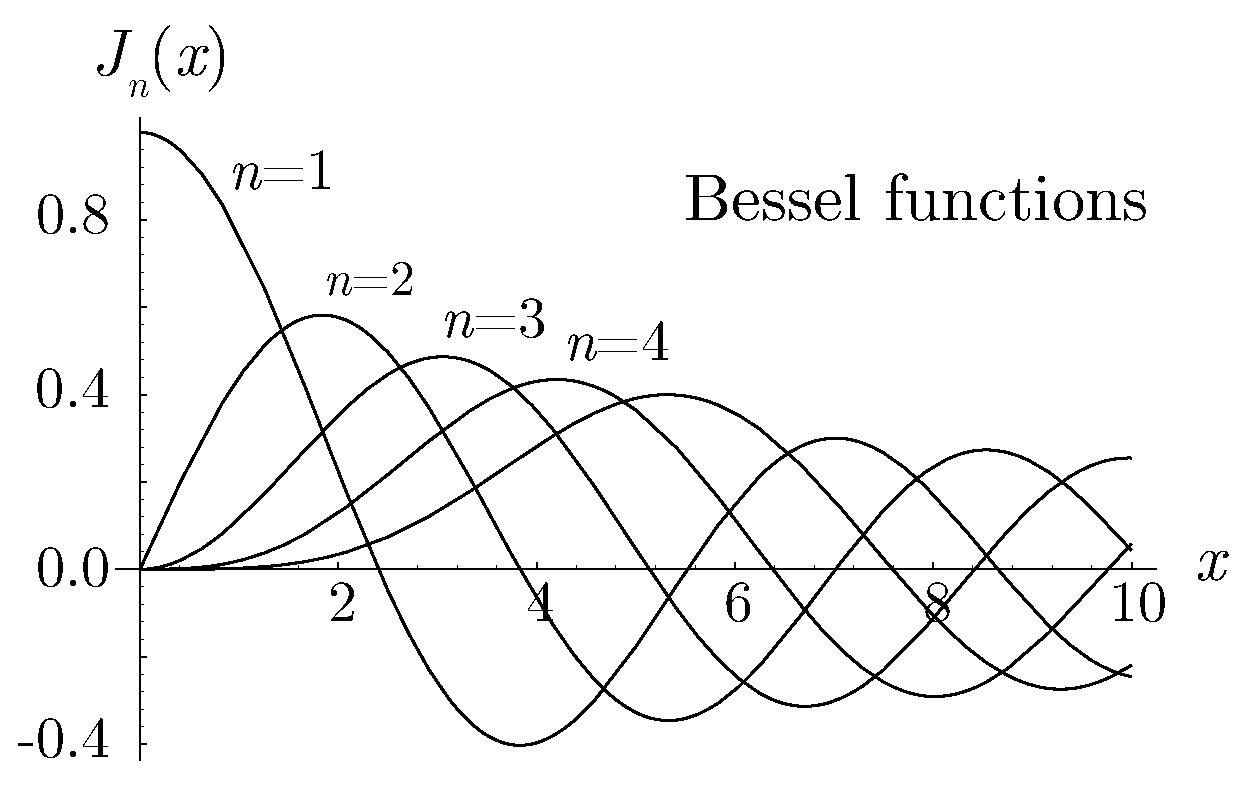
\includegraphics[width=2.0in]{sample.figure.eps} &
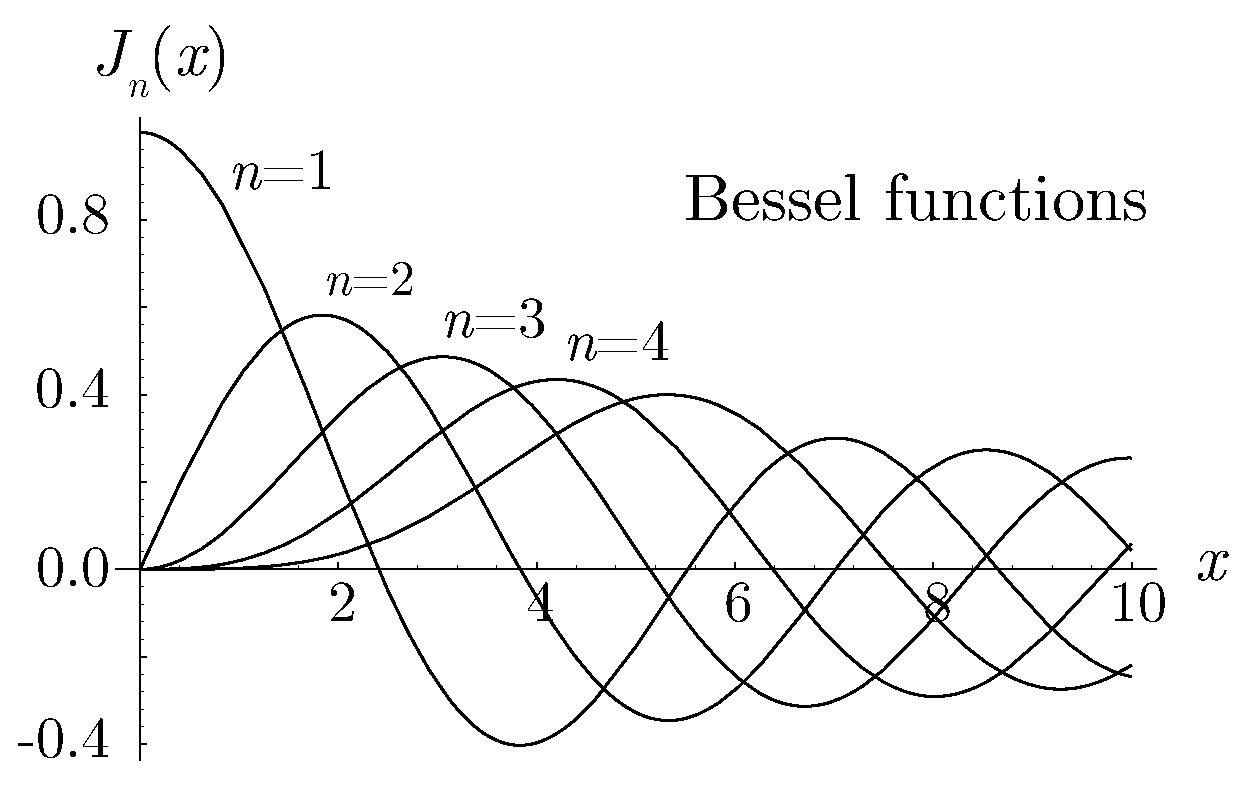
\includegraphics[width=2.0in]{sample.figure.eps} 
\end{array}$
\end{center}
\caption{Sample figure plotting Bessel functions, three times repeated.}
\label{sample}
\end{figure}

\medskip
\leftline{\em Running \LaTeX}
\medskip

You can create a \LaTeX~ file with any text editor ({\tt vi}, {\tt emacs}, {\tt gedit}, 
etc.). 
To get a document, you need to run the \LaTeX~ application
on the text file.  The text file must have the suffix ``{\tt .tex}''.
On a Linux cluster machine, this is done via the command

\medskip
{\tt latex2pdf file.tex}
\medskip

\noindent
This generates {\tt file.pdf}.  You should execute this command at least twice to implement numbering correctly.
Alternatively, you can use {\tt TeXShop} on a Macintosh or {\tt MiKTeX/TeXnicCenter} on a Windows-based machine.
The {\tt .tex} file must have a closing statement as
below.


\end{document}
